\pdfoutput=1

\documentclass{l4proj}

%
% put any packages here
%

\usepackage{listings}
\usepackage{color}

\definecolor{dkgreen}{rgb}{0,0.6,0}
\definecolor{gray}{rgb}{0.5,0.5,0.5}
\definecolor{mauve}{rgb}{0.58,0,0.82}

\lstset{
  language=Scala,
  aboveskip=3mm,
  belowskip=3mm,
  showstringspaces=false,
  columns=flexible,
  basicstyle={\small\ttfamily},
  numbers=none,
  numberstyle=\tiny\color{gray},
  keywordstyle=\color{blue},
  commentstyle=\color{dkgreen},
  stringstyle=\color{mauve},
  breaklines=true,
  breakatwhitespace=true,
  tabsize=2
}

\newcommand{\code}[1]{\texttt{#1}}

\begin{document}
\title{Who To Follow In Context}
\author{Darren Burns}
\date{\today}
\maketitle

\begin{abstract}

%TODO ABSTRACT GOES HERE
abstract here....

\end{abstract}

\educationalconsent
%
%NOTE: if you include the educationalconsent (above) and your project is graded an A then
%      it may be entered in the CS Hall of Fame
%
\tableofcontents
%==============================================================================

\chapter{Introduction}
\pagenumbering{arabic}

%TODO: Include preliminary definitions?

\section{Goal}
The aim of this project was to create an application which provides a relevant set of Twitter accounts to follow based on an input query. In particular, we are interested in recommending accounts which are relevant at the current moment in time. Therefore, a large portion of the project is concerned with providing real-time updates and corrections to recommendations based on the evidence provided via a stream of Twitter statuses.


\section{Motivation}
Guiding users towards the information they require is becoming increasingly important aspect in the development of online services such as social media and e-commerce websites. Without this guidance, users are much less likely to find what they are looking for, and therefore less likely to remain engaged with the service.

The impact of this guidance should not be understated: Celma \& Lamere (ISMIR 2007) noted that 2/3 of movies rented via Netflix were through recommendation, and 35\% of sales made via Amazon are through recommendation. For large companies, this may equate to billions of pounds of additional revenue.

From a social media perspective, recommending interesting people to follow is exceptionally important in retaining users. A Deutsche Bank survey recently showed that the primary reasons people quit Twitter are directly related to the service not meeting their information needs. The top two reasons cited were:

\begin{enumerate}
    \item \textit{``I was getting the information from somewhere else.'' }
    \item \textit{``There was no useful information on Twitter.''}
\end{enumerate}

Hence, by directing users towards Twitter accounts which meet their information needs, it is hypothesised that they are less likely to quit the service. For social media platforms in particular, retaining users is of vital importance since it is directly associated with their primary source of income: advertisements.

Although several products exist today which attempt to solve this problem, they tend to disregard the quickly evolving nature of live events by providing a static set of results. Given the rapidly evolving and sometimes fleeting nature of events, immediate consideration of new tweets may give users insight into how new ``event experts'' emerge as they become relevant, and how that relevance changes over time.

\section{Related Products}

\subsection{Twitter Search}
Twitter's existing search service allows searching for accounts based on a search query. This works similarly to traditional search engines in that the user enters a query and the service returns a list of users that may satisfy the information needs based on that query. This is very similar to the purpose of this project. However, this project displays and updates results in real-time, and new evidence is applied immediately. Therefore if a result page is left open, then the ranking of accounts will be adjusted as people start and stop discussing the query topic. This project intends to provide a live ``window'' into ongoing events, and the frequently updating nature of the displayed results reflects this.

\subsection{Who To Follow at Twitter}
``WhoToFollow'' was the service used at Twitter which recommended accounts to follow based on the people already followed by an account. The primary difference between this project and Twitter's initial Who To Follow system is that this project relies on information retrieval and learning to rank methods which rely entirely on the content of the tweets that users write, whilst Twitter relied on graph analysis, which examines interactions between users to try and identify users similar to those the author already follows. Since the initial deployment of this service in 2010, Twitter announced they are reimplementing the service using Pig and Hadoop to improve scalability, and also to apply machine learning approaches using a wider variety of signals.

\subsection{Klout}
Klout provides a well-known system for ranking the influence of users across numerous social media platforms and online communities. It takes into account over 3600 features from these sources, and processes around 500 million user interactions each day. Although not directly related to this project (Klout ranks users based on a static context: \textit{``How influential is this user?''}), Klout's well documented architecture and popularity in the domain make it worthy of mention.

\section{Relevant Research}

    \subsection{Searching For Quality Microblog Posts}
    %TODO: Discuss
    This paper examines an array of metrics for examining whether a post on a microblog is high quality or not. It introduces an array of features which can be extracted from tweets, and examines the impact of the reputation of external URLs linked to from the tweet. Many of the techniques examined in this paper are applied in the filtering stages of this project, in order to discard tweets which do not meet a threshold on the extracted features.

\chapter{Requirements}

Requirements were gathered during the initial meetings between the author and the project supervisor. These requirements were frequently updated as new considerations were made and new restrictions realised. To ensure the customer (the project supervisor) that progress was being made in satisfying these requirements, weekly status reports were produced during the implementation stage. 

    \section{Functional Requirements}
    
    Functional requirements were gathered in order to describe the specific behaviours the system may offer. In order to prioritise these requirements, the \textit{MoSCoW framework} was used. That is, requirements were categorised in terms of their importance into the sets ``must have'', ``should have'', ``could have'', ``won't have''.
    
    \subsection{Must Have}
    
    Requirements listed in this section were vital to the success of the project. Without satisfying all of these requirements, the project would be regarded as unsuccessful. 
  
    The system itself \textit{must have} the following capabilities:
    \begin{enumerate}
    \item Present a web-based user interface providing querying and result-viewing capabilities.
    \item Read tweets live from the Twitter Streaming API.
    \item Extract the following features from incoming tweets:
        \begin{enumerate}
        \item The length of the tweet.
        \item The number of correctly spelled words in the tweet.
        \item The number of capitalised words in the tweet.
        \item The hashtags used in the tweet.
        \item The number of ``likes'' the tweet had at the time it was processed. 
        \item The number of retweets the tweet had at the time it was processed.
        \item The number of URLs the tweet contains.
        \item The number of users mentioned in the tweet.
        \end{enumerate} 
    \item Filter out Twitter users who post low quality tweets.
   \item Index tweets and relevant metadata so that they can be quickly retrieved given a user query.
    \end{enumerate}

    Additionally, users of the application \textit{must} be able to:
    \begin{enumerate}
    \item Input an event identifying ``hashtag'' into the system.
    \item View the results of the query as they update in real-time.
    \item View the timeline of Twitter accounts suggested by the application, without leaving the application.   
    \end{enumerate}
    
        \subsection{Should Have}
        
        ``Should have'' requirements were considered important for the project, however they are not given the same level of importance as ``must have'' requirements. The exclusion of some of these requirements would not result in an unsuccessful project.
        
        The system \textit{should have} the following capabilities:
        
        \begin{enumerate}
        \item Read historical tweets from a file to improve evaluation capabilities.
        \item When reading tweets from a file, any user timelines viewed should be a snapshot of their timeline corresponding to the time the tweets in the file were sampled from.
        \item Alter its behaviour according to options defined in a configuration file.
        \item Allow users to provide feedback in order to evaluate and improve the relevance of future results.
        \item Provide users with visual feedback to inform them of the current status of the system.
        \item Store tweet features and relevance judgements for evaluation purposes.
        \item Examine a user's timeline to for additional tweets that can be used as evidence for their relevance.
        \end{enumerate}

        \subsection{Could Have}
        ``Could have'' requirements are those that were not considered important, but could improve some aspect of the project such as result relevance or user experience.
        
        The system \textit{could have} the following capabilities:
        
        \begin{enumerate}
        \item Show users any new queries as soon as they are entered in order to encourage interaction.
        \item The reputation of the URLs the tweet contains.
        \item The sentiment of the tweet (e.g. number of positive or negative emoticons used).
        \item Show how user relevance changes over time.
        \item Counts for several punctuation marks used within the tweet. Research has suggested that this may be an indicator of microblog post quality. %TODO: Ref
        \end{enumerate}
        
        \subsection{Won't Have}
        ``Won't have'' requirements are those which the student and project supervisor agreed should not be implemented.
        
        The system \textit{won't have} the following capabilities:
        \begin{enumerate}
        \item Each query should result in a live stream of relevant tweets being displayed alongside the suggested results for that query. This feature was not implemented due to the restriction imposed by Twitter that each application can only have a single stream open.
        \item Provide the ability to ``follow'' users when providing relevance feedback
        \end{enumerate}



    \section{Non-Functional Requirements}
    
    In addition to the functional requirements defined in the previous section, as set of non-functional requirements were agreed on. These requirements describe criteria on how the system should be judged, rather than examining the behaviour it offers. The application was implemented and designed taking these requirements into account as much as possible.
    
    \begin{enumerate}
    \item Support multiple users concurrently without there being a noticeable impact on performance.
    \item Support multiple queries concurrently without there being a noticeable impact on performance.
    \item Be robust enough to handle a variety of issues such as network problems without failing.
    \item Be constructed in a scalable manner so that it can easily be extended to run on a cluster of machines if required in the future.
    \item Be constructed in a maintainable manner.
    \item Display a response (whether that is results or an indication that no results were available) to queries within one second of them being issued.
    \item Operate within the restrictions imposed by the Twitter REST API v1.1 rate limits.

    \end{enumerate}

    

\chapter{System Architecture}

The architecture of the system was designed to adhere to the gathered requirements as far as possible. 

    \section{Server Architecture}
    
    %TODO: Rewrite this to reference the diagram and its individual components. Each subsection should explain the purpose of these components.
On the server side the architecture consists of multiple different components each with their own distinct responsibilities. The design of the server can be seen in Figure \ref{architecture}, and the remainder of this section refers directly to this diagram.

    
    \subsection{Programming Language}
            The server is written using the \textit{Scala} programming language, which is a hybrid of the object-oriented and functional paradigms. Scala was chosen for its lightweight syntax and the fact that it compiles to Java Virtual Machine bytecode, allowing for clean interoperability with existing Java libraries and frameworks. In fact, a number of extremely popular Java libraries are written in Scala, including Apache Spark, Akka, and the Play Framework. Additionally, Scala provides powerful means of asynchronous programming through \code{Future}s and \code{Promise}s, and its \code{Option[T]} type and powerful pattern-matching features make \code{NullPointerException}s impossible since it explicitly requires the developer to check for the possibility that the \code{Option[T]} type contains a \code{None} value. Scala also benefits from its powerful REPL (Read-Execute-Print Loop) which comes bundled with the Scala compiler. This allows developers to immediately evaluate expressions and see the results. Existing code can even be loaded into the REPL so that the effects of performing actions on user defined objects can be examined.
            
        Other languages examined in the initial investigations were Python, NodeJS, and Java. Python was ruled out due to its poor support for concurrency, and its dynamic typing would likely have caused difficulty as the complexity of the project source code increased. NodeJS was considered for its renowned support for real-time web applications. However, the ecosystem surrounding the language has not expanded into the field of processing data streams. As with Python, NodeJS is dynamically typed, and this also factored into the decision to rule it out. Finally, Java was considered due to its unmatched ecosystem of libraries and frameworks and its type system. Java however often requires extra boilerplate code in comparison to Scala. Additionally, Java libraries make excessive use of \code{null} values, which greatly increase the possibility of run-time failure.

    \subsection{Concurrency Model}
    
    The real-time nature of the application means that if performance is poor then it will immediately impact user experience. Should feature extraction for a user timeline take longer than expected, then a user will have to wait until the system gets around to processing that user. As such, high levels of concurrency were deemed vital in order to meet user requests in a timely manner. To accommodate such a requirement, the system was designed using the \textit{Actor model}.
    
    \subsubsection{The Actor Model}

Actor systems provide an alternative means of concurrency that avoid the pitfalls of typical synchronisation methods such as the use of shared mutable state and locks. The actor model of concurrency was first popularised by the Erlang programming language, and has increased in popularity in recent years with the release of applications such as WhatsApp which use the model extensively. An actor system consists of a set of actors. Actors are entities capable of performing some computation on a thread in response to messages. Actors also have the ability to create new “child” actors, and to send messages to other actors in the system, who will then react in their own way depending on the information contained within that message. By communicating between actors solely through asynchronous \textit{immutable} message passing, we guarantee that the computations performed by a single actor cannot result in issues such as thread interference.

\subsubsection{Akka}

    \textit{Akka} is a framework for Scala and Java which implements the actor model. Despite vastly simplifying the concurrency aspect of the implementation, Akka required very little overhead. The actor model framework provided by Akka supports passing approximately 50 million messages per second on an average machine, and around 2.5 million actors can exist per gigabyte of heap space. Each component of the architecture was implemented as an actor, and communication between components in the system was facilitated through message passing.
            
        %TODO: Reword this para and Include Akka-TestKit details
        
        %TODO: Move the following paragraph, it's definitely in the wrong place.
        Despite being primarily used for its concurrency model, Akka provided a number of features ``out-of-the-box'' which satisfied several project requirements. Actors in Akka have a ``supervision strategy'' which defines what actions should be taken when an exception occurs within them. This allows the system to meet the high degrees of fault tolerance and resilience required. The default supervision strategy (simply restarting the actor when an exception occurs) solved many issues that were encountered. For example, it was common for the Twitter streaming API to become unavailable and an exception was therefore thrown. The actor handling the stream was automatically restarted and the stream handle resent to all of the actors that required access to it. No explicit error handling code was required, yet the application was able to self-heal and become fully functional as soon as the streaming API became available again.

        \subsection{Reactive Systems}
        The architecture of the system is implemented to conform to many of the tenets described in the ``Reactive Manifesto''. That is, the system architecture is designed to be responsive, resilient, elastic, and message-driven.
        
            \subsubsection{Responsiveness}
            Responsiveness is a key aim of the application. Messages passed from actor to actor in potential bottlenecks are load-balanced in order to minimise the work queued on a single actor or thread and maximise throughput. Within each defined actor is a response time guarantee which, if not met, causes the actor to be restarted in attempt to regain responsiveness. 
            
            \subsubsection{Resilience}
            The application provides the guarantee of resilience through ``self-healing''. Should an actor executing some computation encounter an exception, its parent is notified and takes the appropriate action in order to cleanly recover. Additionally, if an exception occurs within any actor, it is treated in isolation, and other actors are not affected unless the parent actor's supervision strategy explicitly calls for it. Therefore, problems are compartmentalised and only closely related actors are affected.
            
            \subsubsection{Elasticity}
            Some actors within the system are implemented as state machines with the ability to change their behaviour at run-time, in response to certain events. This can be useful, for example, if the application hits the Twitter API rate-limit. The behaviour of the corresponding actor can be modified to stop making API requests for a specified period of time, and then modified back to its original API-reliant behaviour after this time period has expired.
            
            \subsubsection{Message-Driven}
            The application is entirely message driven. The root messages are batches of tweets read from a stream of tweets, or user interactions with the system. Each of these messages results in a chain of messages being sent asynchronously between actors as they handle the situation.       
        
        \subsection{Dependency Injection}
        
        The system relies heavily on the \textit{dependency injection} design pattern. This pattern greatly reduces coupling between components, and enforces a separation of concerns by separating dependency creation from behavioural code.
        
            \subsubsection{Google Guice}
                
        \textit{Google Guice} is a dependency injection framework for Java which manages the dependency graph that exists between objects in an object-oriented environment. Using Guice, one can request an instance of an object when required by ``injecting'' the instance into a ``setter'' method or a constructor.

Guice was primarily used for the injection of actor references into other actors. If we ever wish to send a message to an existing actor in order for it to perform some computation, we simply ask Guice for the instance of the required actor by injecting the actor into the constructor of the current class using the \code{@Inject} and \code{@Named} annotations provided by the framework.

%TODO: Add code snippet showing how Guice was used in the injection of actors. (Add this snippet in implementation)
        
        \subsection{Feature Extraction and Filtering}
        Incoming tweets are initially passed into the feature extraction component. \textit{Spark Streaming} (and Twitter4j for authentication purposes) provided a convenient way to access the Twitter streaming API, and distribute the feature extraction workload across multiple processing cores. Spark is designed to work in a distributed environment, and therefore also leaves open the possibility of distributing the stream across multiple machines in a cluster should the need arise.
        
        This component extracts statistics from the content of the tweet and its metadata. These features are passed to the filtering component which will discard tweets which do not meet a configurable quality threshold. The purpose of filtering these tweets is to prevent unnecessary computational load and also to avoid hitting the rate limiting restrictions of the Twitter API.
        
        After low quality tweets have been filtered, the features of the remaining tweets are stored for future use, and the remaining tweets are progressed to the indexing stage of the pipeline.

Both the feature extraction and filtering components may receive tweets from other locations within the system. If the system ever deems a user to be relevant (for example, if they appear in a result stream for an open channel, or a user of the system views their profile), then the tweets present on that user’s timeline are fed back into the pipeline in order to extract further evidence in the hopes of improving the relevance of results.

        \subsection{Feature Storage}
        
        Two different technologies provide the persistance layer for the application. Each of these provide different benefits and so the decision of which to use and where varied depending on context.
        
        \subsubsection{Redis}
        \textit{Redis} is an in-memory data structure storage engine which is used for storage of extracted features. By keeping data in memory it enables quick reads and writes. Its built in data structures simplified the implementation of certain features. For example, a Redis SortedSet data structure is used for the calculation of the median time since the user last made use of the query term as a hashtag. Since the application must process vastly more reads than writes for individual users, allowing Redis to perform the sorting step at write time make the system more efficient than if we were required to sort an array each time the latest results were retrieved for a user.
        
         \subsubsection{MongoDB}
         \textit{MongoDB} is a NoSQL database used for the caching of Twitter user metadata in order to reduce the number of API requests required. For example, we store the URL of the user's profile picture and timeline colour in MongoDB and check for its existence here before making an additonal API request for the information. We also store user relevance feedback in MongoDB for evaluation purposes.
         
         NoSQL was used due to the lack of need of relational features. Each category of item stored in this database was entirely independent from the others, and thus guaranteed that relational database tools such as joins would not be necessary.


        \subsection{Indexing and Retrieval}
        After low quality tweets have been discarded, those remaining are sent to the indexer where they will be stored for efficient retrieval. 
        
        When a query is received, the Query Service will construct a result stream between the information retrieval engine and the user who entered the query. The information retrieval engine will then be frequently polled for new results, and the new results will be sent to the user as soon as they are available.
        
            \subsubsection{Terrier Information Retrieval Platform}
            Both indexing and retrieval capabilities are provided by the \textit{Terrier Information Retrieval Platform}. Terrier's \code{MemoryIndex} allowed an index to be maintained online, and thus was the technology which enabled results to be displayed and updated in real-time.
       
        \subsection{Metrics Reporting}
        Throughout different stages of the pipeline, different metrics can be collected. These metrics are both logged and sent to the user in real-time to provide insight into the operation of the system. This is important as it ensures the user that the system is working as expected. If a large period of time passes and no new users have appeared in the stream of results they are viewing, they might think that something has went wrong. By keeping them constantly updated on the number of users the system has seen, they are ensured that it is working as expected.
        
        Numerous different technologies were examined for providing this functionality, including the \textit{Comet model} in HTTP 1.X, the WebSocket protocol, and using the persistent connection and multiplexing capabilities of HTTP 2.0.
        
        Comet sockets were introduced to provide streaming capabilities before the introduction of the WebSocket API, and as such rely on many browser hacks to work properly. However, with the correct hacks this provides excellent compatibility with older browsers which do not support WebSockets. Facebook Messenger is one such service that (as of 2013) relied on Comet for providing real-time notification and chat.
        
        HTTP 2.0 is the latest version of the HTTP specification which provides an abundance of new features and exceptional performance improvements over the currently dominant HTTP 1.X protocols. These features (such as connection multiplexing) mean that the ``hacks'' required with the first version of the protocol which enable streaming are no longer required. However, support for HTTP 2.0 in existing libraries and frameworks are limited as of the time of writing. As such, relying on HTTP 2.0 would have added too much development overhead to make it practical.
        
       After consideration of the above technologies, the WebSocket protocol was chosen to enable real-time communication between the server and connected clients. The WebSocket protocol is well supported in modern browsers, and is specifically designed for immediate communication between servers and clients. Additionally, WebSockets are well supported in modern web frameworks meaning there is a large community of developers  and supporting documentation available.
          
        A downside of using a WebSocket reliant architecture is that the protocol is much slimmer than HTTP, and therefore it was required to implement the notion of a ``keep-alive'' to ensure that channels are cleaned up in the case that no client registers an interest in it.
        
                \subsubsection{Play Framework}
        The \textit{Play Framework} was used for its WebSocket implementation and to create REST API endpoints, such as the endpoint used in fetching the timeline and metadata for a user when they are clicked on in a result set. Since routing and rendering was done on the front-end, only a small subset of the features of Play were required. This framework provided the benefit of having excellent integration with Akka (Play is also written using Akka) and Guice, allowing WebSocket connections to be accepted using actors. An additional benefit of using this framework is that it is one of the most popular web frameworks for Java and Scala, and as such it has an active developer community with clear and extensive documentation.
        
\begin{figure}
\centering
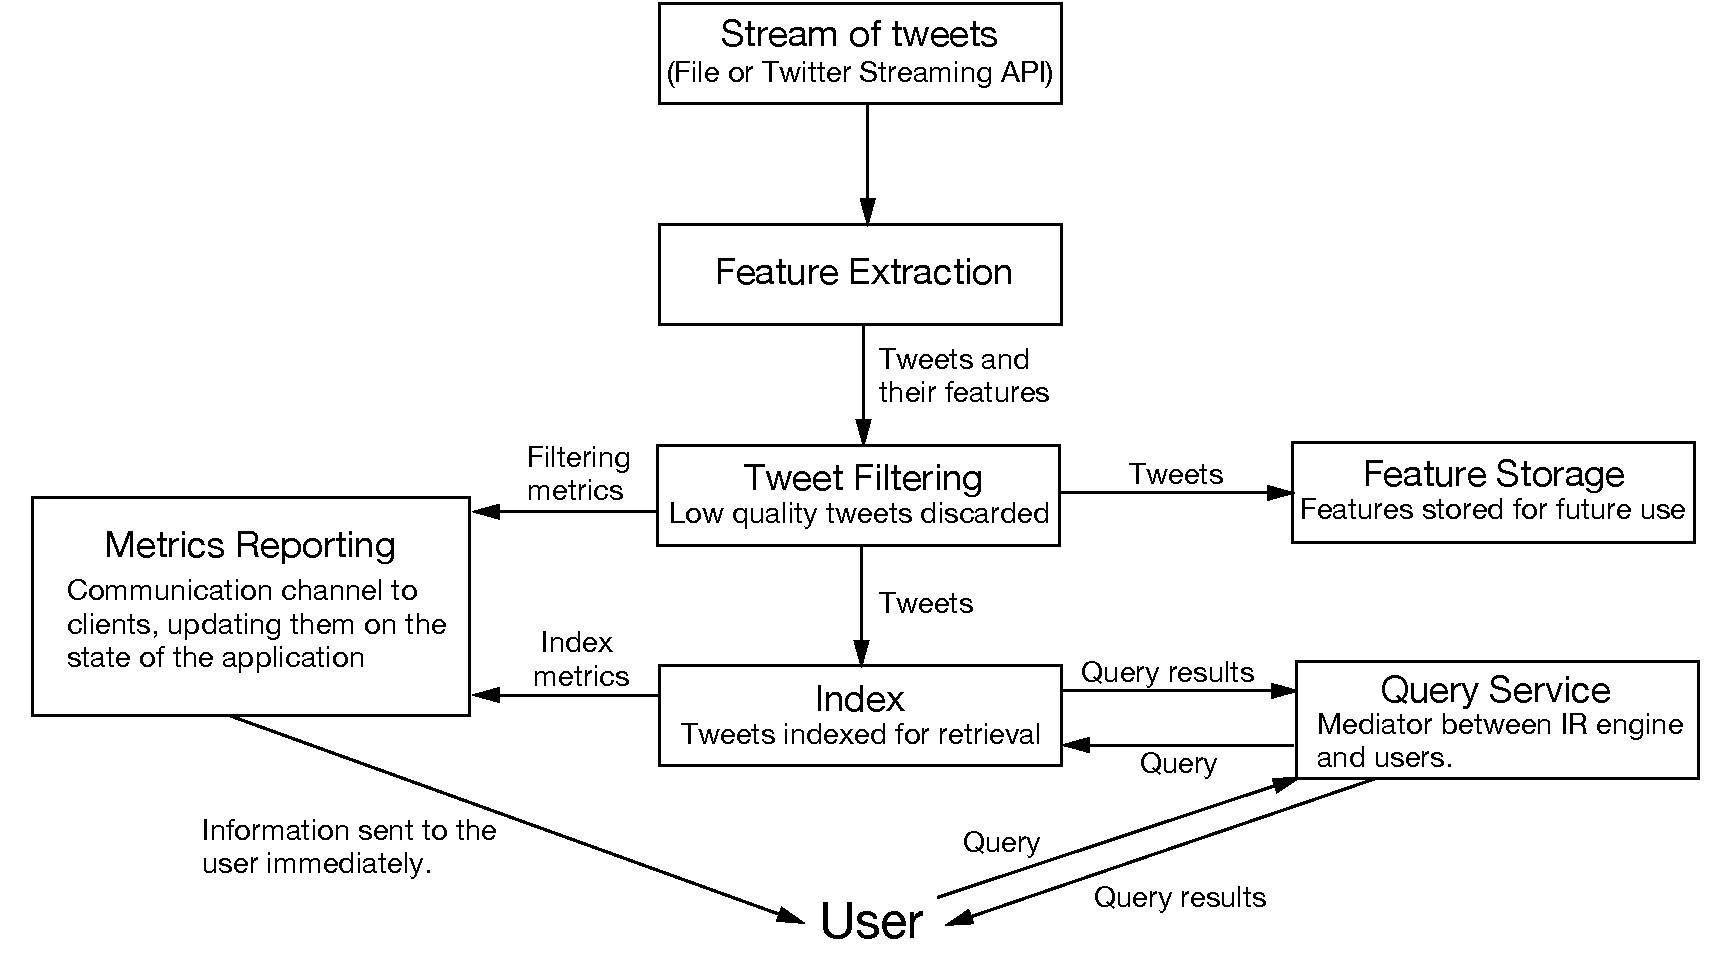
\includegraphics[height=278px,width=496px]{architecture.pdf}
\caption{The high-level architecture of the system. The ``Implementation'' chapter looks at the internal workings of each component in detail.}
\label{architecture}
\end{figure}




        
    \section{Front-End Architecture}
    
        \subsection{Programming Language}
        The programming language used to create the front-end of the application was \textit{TypeScript}. TypeScript is a typed superset of JavaScript which provides compile-time type checking which eliminates a large number of run-time errors. Existing JavaScript libraries can be used from within TypeScript by including a ``type definitions'' file in the project. The purpose of such files is to provide a mapping from the non-typed JavaScript constructs to their corresponding TypeScript types.
        
        The front-end was initally written in JavaScript and then migrated to TypeScript as the number of type related errors began to increase due to the increasing complexity of the front-end. Although the initial migration to TypeScript was extremely time consuming, the number of run-time errors encountered significantly decreased. Since TypeScript is a type checked language, we also gain the benefits of code-completion and refactoring capabilities within certain integrated development environments.
    
        \subsection{Single-Page Application}
    %TODO: These are implementation details...?
    The client side of the application is constructed as a single-page application (SPA) meaning that the entire application is mounted at a single URL (excluding API endpoints which return JSON rather than text/html content). Navigation between pages is then managed entirely by client-side code. Additionally, the entirety of the views are implemented on the client side, and data is fetched either via a REST API (as opposed to server-side rendering of views) or through an open WebSocket. 

This approach provides the benefit of reducing the number of requests made to the server, and greatly improves the responsiveness of the front-end. 

Although we gain an overall more responsive experience using this architecture, it does have some associated flaws. The initial page load is often slower, since the client contains more code than it otherwise would if rendering and routing was managed on the server. Additionally, the improvement in page load times can place a burden on the server, since it has to ensure that the data will be available when a user requests it. If the data is not available when required by the user, it may prove irritating as they wait on certain portions of the interface to update.

    \section{Component-Based Design}

        \textit{React} is a JavaScript library developed by Facebook for constructing user interfaces in a component-based fashion. There is an abundance of modern libraries and frameworks for developing user interfaces. React was chosen primarily for its enforcement of the idea of ``separation of concerns'' and its renowned performance.
        
        The other popular client library considered for the project was AngularJS by Google. However, Angular is framework rather than a library and as such forces the developer to write their application within its restrictions.

        \subsubsection{React Router}
        The decision to make routing a concern of the front-end was driven by the existence of \textit{React Router} and the fact that the application view has a limited number of overall states. Using this library allowed views to be declared hierarchically, so that only required subtrees of the view are re-rendered on a URL change.
        %TODO: Finish this
        
        %TODO: Discuss elemental/material-ui and react-velocity and it proved helpful i.e. visual cues preventing confusion etc.
        



% TODO: Include diagrams showing the structure of the front-end and back-end architectures.


\chapter{Implementation \& Design}
                    

\section{Server Implementation}

    \subsection{Tools \& Practices}
    
             \subsubsection{Git}
         \textit{Git} is a distributed version control system which was used extensively during the development of the project. A working implementation of the project was always maintained on the \code{master} branch. Features were developed on their own branches so as to not interfere with \code{master}.
         
             \subsubsection{GitHub}
             The project is also linked to a remote repository hosted on \textit{GitHub}.
             
             \subsubsection{Agile Software Development}
             The \textit{Agile} software development process was followed throughout the lifetime of the project. Although there was an initial requirements gathering stage, these requirements frequently changed, and the product itself changed as a result.
             
             \subsection{Kanban \& Trello}
             Project task management was done using the ``Kanban'' system, where projects are represented as a set of named lists and cards. \textit{Trello} is an online platform which implements this system, and was used extensively throughout all stages of the project.
         
             \subsubsection{SBT (Scala Build Tool)}
         \textit{SBT} is a build management system commonly used in Scala projects which is similar to popular Java build tools such as Maven and Gradle. SBT was used in the project to maintain and resolve dependencies, run tests, and to build and run the project.

    
% Each subsection should be modelled around one of the components mentioned in the requirements section. 
    
    \subsection{Feature Extraction}
        
        Spark Streaming provides us with a \code{ReceiverInputDStream[Status]} (discretised stream) representing the incoming stream of tweets. The tweet stream was mapped to a ``windowed'' tweet stream. This allows us to view the stream through a ``sliding window'', and perform operations on these individual windows of tweets. The tweets in each window are batched and sent through the rest of the pipeline together. The width of the sliding window is defined temporally, as is shown in Figure \ref{slidingwindow}.
        
\begin{figure}
\centering
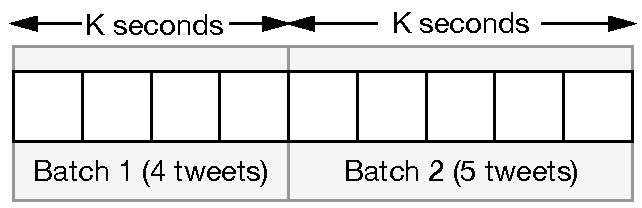
\includegraphics[scale=0.8]{slidingwindow.pdf}
\caption{Tweets are batched temporally and sent throughout feature extraction together.}
\label{slidingwindow}
\end{figure}

        The \code{FeatureExtraction} actor maps our windowed stream of tweets into a windowed stream of tweet features, which is immediately filtered to discard those tweets which do not meet the threshold quality criteria. These features are then sent to Redis for storage, and the original status is sent to the indexing actor for storage in a Terrier \code{MemoryIndex}.
        %TODO: The following paragraph holds for now, but if I implement the 'trending' thing then it will no longer be relevant.
                Treating the stream as a time-based sliding window also allows us to answer questions such as \textit{``which users have most frequently used hashtag H within the past N minutes?''}. Despite the application having the ability to answer such questions, this feature remains unused in the current iteration and remains solely as a potential area for future expansion. 
        
        In early iterations of the project, features were stored in MongoDB. However, this proved to be a bottleneck on performance, since the implementation was unable to keep up with the rate at which new features were calculated. There are several reasons which explain why this situation occurred:
        
        \begin{itemize}
        \item MongoDB persists data on disk, resulting in slow read/write times compared to in-memory solutions.
        \item An asynchronous MongoDB driver was not used and so blocking occurred frequently.
        \item Parallel insertions were not used. The MongoDB Scala driver had no serialisation/deserialisation support and this made using the parallel insertion API overly cumbersome.
        \end{itemize}
        
        To overcome this bottleneck Redis was employed as the storage engine for features. This resulted in immediate performance improvements, but the system was still unable to store features at the rate they were being generated. Three additional steps were taken in order to ensure that features were persisted at an acceptable rate:
        
        \begin{itemize}
        \item Connection pooling was used to ensure that the application did not have to reconnect to the Redis server on each operation.
        \item Requests to read and write features from Redis were partitioned by defining a \code{RedisRequest} type with two subtypes: \code{RedisReadRequest} and \code{RedisWriteRequest}. This allowed for the separation of reads and writes so that they can be processed by separate worker pools.
        \item Read and write requests were sent to a ``routing'' actor (named \code{RedisActor}) which maintains two pools of actors: one pool containing workers which deal with reading and unmarshalling data from Redis, and one containing workers which handle storing new features to Redis. These requests are distributed to workers using a Round-Robin algorithm, to ensure that the work is evenly distributed. Figure \ref{loadbalancing} shows how tasks were distributed between workers to maximise concurrency.
        \end{itemize}


\begin{figure}
\centering
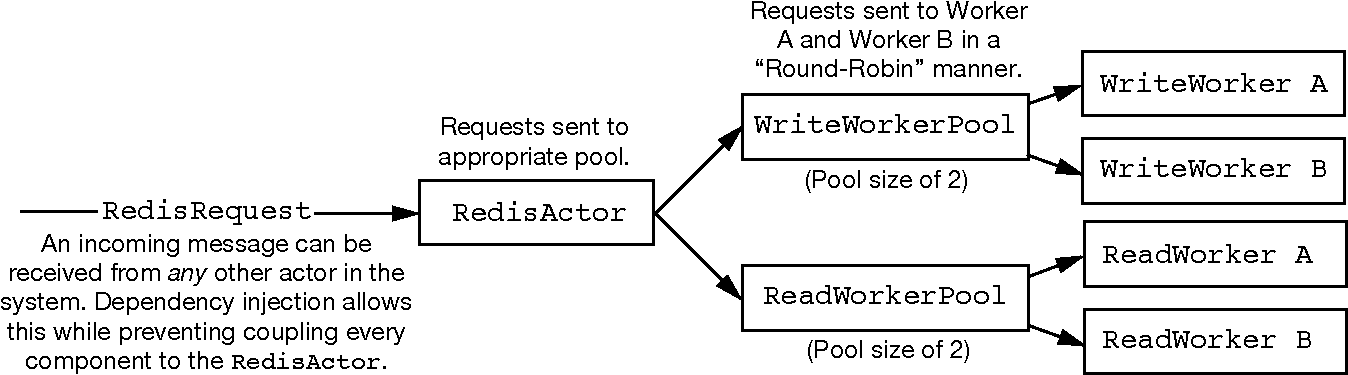
\includegraphics[scale=0.7]{loadbalancing.pdf}
\caption{An example of how requests were load-balanced in order to prevent overworked actors and maximise concurrency. This is a lower level view into the inner workings of the ``Feature Storage'' component shown in Figure \ref{architecture}}
\label{loadbalancing}
\end{figure}
        
        Akka made implementation of this load balancing simple since it provides extensive built-in support for such tasks, including protocols much more advanced than the Round-Robin method used in this component. The code for implementing a worker pool was a single line, as can be seen in the code for creating the \code{WriteWorkerPool} shown below.
        
        \begin{lstlisting}
          val writingWorkerPool = context.actorOf(RoundRobinPool(4)
                .props(Props[RedisWriterWorker]), "writingWorkerPool")
        \end{lstlisting}

        
        After implementing the feature storage component using these techniques, it was found that it no longer restricted overall system performance.

        \subsection{Indexing}
        %TODO: Should I go into details on what indexing is and show how the tweets are stored?
        Tweets received at the indexing component are stored in a Terrier \code{MemoryIndex}. Each document stored in the index consists of one or more tweet from a single Twitter user. If a tweet appears in the stream authored by a user that we have not seen before then we store the author's username, screen name, and profile biography in a Terrier metadata index so that it can be quickly retrieved in the case that the document is returned in response to a query.        
        
        \subsection{Retrieval}
        %TODO: This was previously in the architecture section but its actually an implementation detail of the "Search Component" described in the architecture section. It has to be completely reworded.
        
        %TODO: Discuss keep-alive implementation
        To maximise performance, it was important to ensure that two users entering the same query does not result in the system computing the same stream of results twice. The traditional means of preventing this is through caching query results. Unfortunately, caching is not as practical in a system that is performing real-time indexing and providing results as a stream, since the results of a query change so frequently.
        
        To get around this limitation, we map each new query to a ``channel'', that the results of that query are forwarded through. When a user inputs a query to the system, they are connected to a channel and will see the same stream of results for that query as any other user who has entered the query. If the channel corresponding to their query does not already exist, then it is created. Figure \ref{channels} gives a simplified example of what the clients/channels relationship may look when the system is running.
        
        When a channel is created, it registers a scheduled message to poll Terrier for the latest result set in a configurable interval. The code below shows how the polling rate was read from a dependency injected configuration file in a way that avoids \code{null} values, and then used to schedule the channel's work.
        
        \begin{lstlisting}
          // Read the polling duration from the config file  
          val resultPollDuration = config.getInt("results.pollingrate").getOrElse(1000)
          
          // Schedule the requests for the latest query results
          val fetchTick = context.system.scheduler
                .schedule(Duration.Zero, FiniteDuration(resultPollDuration, TimeUnit.MILLISECONDS), self, FetchLatestQueryResults)
           
        \end{lstlisting}

        Through repeated polling, the result sets obtained from Terrier were transformed into a stream of results sent to clients.
        
        Channels will remain open for a query for as long as at least one user is connected to the result stream. In order to determine whether any user is interested in the channel, connected users automatically send special ``keep-alive'' messages that the server interprets as a user expressing a desire to keep the channel open. Each open channel monitors the timestamp associated with the latest keep-alive receieved, and will free its associated resources if the latest keep-alive is ever older than some configurable threshold. In this way we ensure that a channel is never closed while a user is viewing a stream of results. Using this technique also allows us to close result streams when they are no longer required and therefore prevents resource leaks.
        
    \subsection{Metrics Reporting}
    This component is implemented as a single actor which can receive data from any other component in the system. By sending information to this actor, and specifying how it should translate this information (e.g. a Scala case class) to JSON, it allows any component to communicate with the client. The code below provides an example of how messages received at this actor are examined using Scala's pattern matching and simply forwarded through a channel which all users are connected to by default.
    
    \begin{lstlisting}
      override def receive = {
        case numUsers @ NumberOfUsersSeen(_) => 
            channelMeta.channel push Json.toJson(numUsers)
        ...
      }
    \end{lstlisting}

The code which maps user-defined Scala types to valid JSON relies on the Play Framework's ``Writes'' converters. The converter for the example above is shown below:

    \begin{lstlisting}
      implicit val numberOfUsersSeenWrites = new Writes[NumberOfUsersSeen] {
        def writes(numberOfUsersSeen: NumberOfUsersSeen) = Json.obj(
            "numUsersSeen" -> numberOfUsersSeen.numUsers
        )
      }
    \end{lstlisting}

    
        
\begin{figure}
\centering
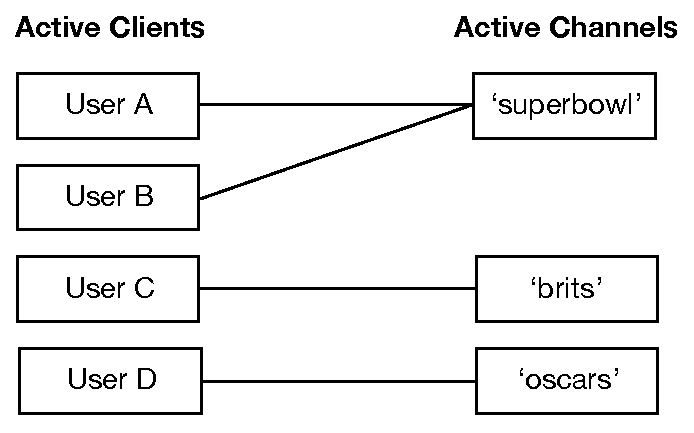
\includegraphics[scale=0.75]{channels.pdf}
\caption{\textit{An example of the one-to-many relationship that exists between users and channels}. Users A and B both connect to a single channel after entering the same query (``superbowl''), and will receive the results it outputs. This channel will perform the exact same actions regardless of the number of users connected.}
\label{channels}
\end{figure}        
                          
\section{Client Implementation}
    %TODO: Write this section - include timeline of UI development
        \subsection{Tools \& Practices}
           %TODO: Add testing framework information

        \subsubsection{Gulp}
        \textit{Gulp} is a front-end build system which was used to speed up parts of development. Gulp tasks were defined to watch TypeScript files for changes and automatically transpile them into new JavaScript files using the ``tsc'' TypeScript compiler.
        
        \subsubsection{Node Package Manager}
        \textit{Node Package Manager} (NPM) was used to manage front-end dependencies. By specifying these dependencies in a \code{package.json} file, developers can simply run \code{npm install} to fetch all of the requirements for the application. NPM was used in conjunction with the \textit{TypeScript Definition Manager} which fetches TypeScript type declaration files.
        \subsection{User Interface}
        %TODO: Remember to discuss responsive design, animations used for specific reasons
        The user interface was one of the most heavily iterated upon aspects of the application. Using a component-based user interface framework allowed components to be iterated on in isolation, and so changing the UI could be done gradually to allow for progress on other features.
        
        \subsection{Searching}
        TODO Entering a query opens a new channel and schedules a keep-alive to be...
        
        \subsection{Query Results}
        TODO Discuss presentation of query results - single page to encourage users to view lower ranked profiles. Also shows more clearly changes in rankings, since users can never 'fall off' the first page. Spark lines showing changes in individual users gives insight into changes in user relevance which doesnt fit the typical trend.
        
        \subsection{Recent Queries}
        TODO Discuss animation
        
        \subsection{Previewing Twitter Users}
        TODO Discuss layout, reason for animation, flexbox usage, usage of profile colours - how relevance marking button colours work (tinycolor)... 
        
        
\chapter{Evaluation}
%TODO: Write evaluation

\section{Experiments}
    
    \subsection{Investigations on Filtering Controls}
    How does filtering affect relevance judgements, percentage of users filtered, etc. Even just applying a restriction that users have a spelling accuracy gt 0.5 meant discarding like 90 pc of users.
    
    \subsection{Investigating the Effects of Stream Replay Rate}
    The rate at which tweets are read when using a source file has a direct effect on system performance and usability. An investigation was conducted into the performance and usability impact of altering the stream replay rate.

\section{User Evaluation}

    In addition to weekly feedback from the project supervisor, a user evaluation study was conducted in the final weeks of the project.

    \subsection{Questionnaires}
    Pre and post evaluation questionnaire results discussion..

    \subsection{Usability Study}
    Computer usability questionnaire, think-aloud during evaluation to determine issues encountered...
    
    \subsection{Relevance Judgements}
    What users thought of results, did they make relevance judgements often?

\section{Behaviour Testing}
    %TODO: Change section title to include behavioural tests if Jest is used.
    \subsection{Server}
    Testing on the server...
    
    \subsection{Client}
        The front-end of the application was tested using the \textit{Jest} testing and mocking library...
        
        
\section{Integration Testing}
    In addition to tests which ensure that components behave as expected, tests were also written to ensure that they work correctly within their intended environment. In the context of actor systems, this is done by testing how actors respond to \textit{stimulus} from a \textit{probe}. Since actors perform computation in response to messages, we can probe their behaviour by sending them test messages and ensuring that they respond as expected.
    
    As an example of how integration testing was useful: When a \code{SparkContext} has been started, it is illegal to attempt to register additional actions on the data. Since the system registers Spark actions in asynchronous calls, it is a possibility that the \code{SparkContext} is started before all actions are registered. To avoid this scenario, any actor registering Spark actions must inform its parent when it has done so. The parent will wait for all child actors to make this confirmation before starting the context. Integration testing is used to ensure that all actors which register Spark actions correctly inform their parent when this registration is complete, and thus avoids a runtime \code{IllegalStateException}.
    
    

\section{Performance Testing}

    \subsection{Actor Message Response Time Testing}

    \subsection{Server Throughput Testing}
    %TODO: Use BlazeMeter.

    %TODO: Use Chrome devtools for paint regions, profiling 'jank' etc.
    \subsection{Profiling Client Side Performance}
    
    
    765 rules (95\%) of CSS not used by the current page.
    
    Use Chrome devtools and painting and profiling info here... Read the Google Developers tutorial again.
        
    
    



\chapter{Conclusions \& Future Work}

    %TODO: Acknowledgements
    
    %TODO: Not all requirements were met - some features required weren't extracted for example.

    %TODO: Machine learning approach for user filtering rather than heuristic filters
    
    %TODO: Feeding evaluation results into learning to rank technique

%%%%%%%%%%%%%%%%
%              %
%  APPENDICES  %
%              %
%%%%%%%%%%%%%%%%
\begin{appendices}

\chapter{Running the Programs}
An example of running from the command line is as follows:
\begin{verbatim}
      > java MaxClique BBMC1 brock200_1.clq 14400
\end{verbatim}
This will apply $BBMC$ with $style = 1$ to the first brock200 DIMACS instance allowing 14400 seconds of cpu time.

\chapter{Generating Random Graphs}
\label{sec:randomGraph}
We generate Erd\'{o}s-R\"{e}nyi random graphs $G(n,p)$ where $n$ is the number of vertices and
each edge is included in the graph with probability $p$ independent from every other edge. It produces
a random graph in DIMACS format with vertices numbered 1 to $n$ inclusive. It can be run from the command line as follows to produce 
a clq file
\begin{verbatim}
      > java RandomGraph 100 0.9 > 100-90-00.clq
\end{verbatim}
\end{appendices}

%%%%%%%%%%%%%%%%%%%%
%   BIBLIOGRAPHY   %
%%%%%%%%%%%%%%%%%%%%

\bibliographystyle{plain}
\bibliography{bib}

\end{document}
